\chapter{Конструкторский раздел}
\label{cha:design}

\section{Схемы алгоритмов}
В данной части будут рассмотрены схемы алгоритмов сортировки пузырьком, вставками и выбором. На рисунках \ref{fig:scheme_bubble}, \ref{fig:scheme_insert}, \ref{fig:scheme_select} представлены рассматриваемые алгоритмы.


\begin{figure}[h]
    \centering
    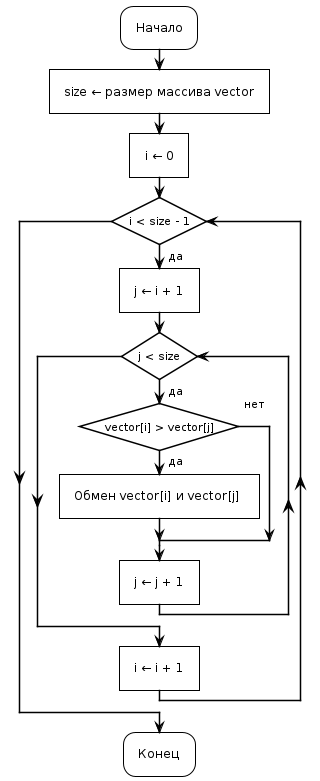
\includegraphics[width=0.3\columnwidth]{plantuml/bubble.png}
    \caption{Схема алгоритма сортировки пузырьком}
    \label{fig:scheme_bubble}
\end{figure} 

\begin{figure}[h]
    \centering
    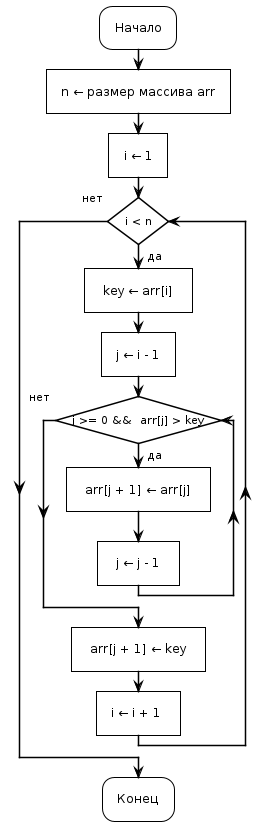
\includegraphics[width=0.3\columnwidth]{plantuml/insert.png}
    \caption{Схема алгоритма сортировки вставками}
    \label{fig:scheme_insert}
\end{figure} 


\begin{figure}[h]
    \centering
    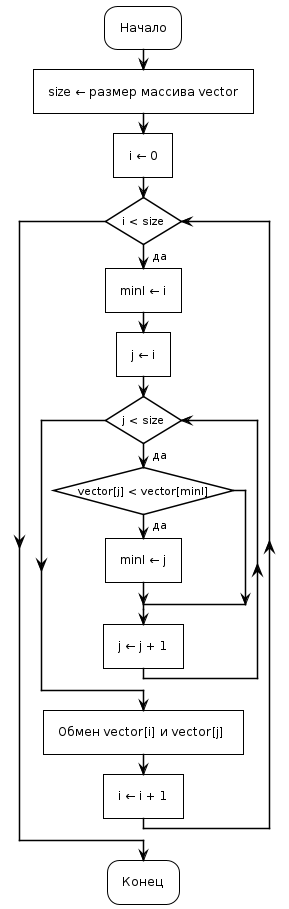
\includegraphics[width=0.3\columnwidth]{plantuml/select.png}
    \caption{Схема алгоритма сортировки выбором}
    \label{fig:scheme_select}
\end{figure} 

\clearpage
\section{Трудоёмкость алгоритмов}

\subsection{Модель вычислений}

Для последующего вычисления трудоемкости необходимо ввести модель вычислений. Трудоемкость "элементарных" операций оценивается следующим образом:

\begin{enumerate}
	\item Стоимость операций $+,-,=,<,>,\geq, \leq, ==, -=, +=, ++, --, [\space], \&\&, ||, >>, <<$ оценивается в 1 пункт
    \item Стоимость операций $*, /, \% $ оценивается в 2 пункта

	\item Трудоемкость оператора выбора if условие then A else B рассчитывается, как (\ref{for:if}).
	\begin{equation}
	\label{for:if}
	f_{if} = f_{\text{условия}} +
	\begin{cases}
	f_A, & \text{если условие выполняется,}\\
	f_B, & \text{иначе.}
	\end{cases}
	\end{equation}
	\item Трудоемкость цикла рассчитывается, как (\ref{for:for}).
	\begin{equation}
	\label{for:for}
	f_{for} = f_{\text{инициализации}} + f_{\text{сравнения}} + N(f_{\text{тела}} + f_{\text{инкремента}} + f_{\text{сравнения}})
	\end{equation}
	\item Трудоемкость вызова функции равна 0.
\end{enumerate}

Пусть размер массивов во всех вычислениях обозначается как $N$.

\subsection{Алгоритм сортировки пузырьком}

Трудоёмкость алгоритма сортировки пузырьком состоит из:
\begin{itemize}
	\item трудоёмкость сравнения и инкремента внешнего цикла $i \in [1..N)$ (\ref{for:bubble_outer}):
	\begin{equation}
	\label{for:bubble_outer}
	f_{i} = 2 + 2(N - 1)
	\end{equation}
	\item суммарная трудоёмкость внутренних циклов, количество итераций которых меняется в промежутке $[1..N-1]$ (\ref{for:bubble_inner}):
	\begin{equation}
	\label{for:bubble_inner}
	f_{j} = 3(N - 1) + \frac{N \cdot (N - 1)}{2} \cdot (3 + f_{if})
	\end{equation}
	\item трудоёмкость условия во внутреннем цикле (\ref{for:bubble_if}):
	\begin{equation}
	\label{for:bubble_if}
	f_{if} = 4 + \begin{cases}
	0, & \text{в лучшем случае}\\
	9, & \text{в худшем случае}\\
	\end{cases}
	\end{equation}
\end{itemize}

Трудоёмкость в \textbf{лучшем} случае (\ref{for:bubble_best}):
\begin{equation}
\label{for:bubble_best}
f_{best} = \frac{7}{2} N^2 + \frac{3}{2} N - 3 \approx \frac{7}{2} N^2 = O(N^2)
\end{equation}

Трудоёмкость в \textbf{худшем} случае (\ref{for:bubble_worst}):
\begin{equation}
\label{for:bubble_worst}
f_{worst} =  8N^2 - 8N - 3 \approx 8N^2 = O(N^2)
\end{equation}

\subsection{Алгоритм сортировки вставками}

Трудоёмкость алгоритма сортировки пузырьком состоит из:
\begin{itemize}
	\item трудоёмкость сравнения и инкремента внешнего цикла $i \in [1..N)$ (\ref{for:isort_outer}):
	\begin{equation}
	\label{for:isort_outer}
	f_{i} = 2 + 2(N - 1)
	\end{equation}
	\item суммарная трудоёмкость внутренних циклов, количество итераций которых меняется в промежутке $[1..N-1]$ (\ref{for:isort_inner}):

	\begin{equation}
	\label{for:isort_inner}
	f_{if} = 4 + \begin{cases}
		0, & \text{в лучшем случае}\\
		3(N - 1) + \frac{N \cdot (N - 1)}{2} \cdot (3 + f_{if}), & \text{в худшем случае}\\
	\end{cases}
	\end{equation}

	\item трудоёмкость условия во внутреннем цикле (\ref{for:isort_if}):
	\begin{equation}
	\label{for:isort_if}
	f_{if} = 4 + \begin{cases}
	0, & \text{в лучшем случае}\\
	9, & \text{в худшем случае}\\
	\end{cases}
	\end{equation}
\end{itemize}

Трудоёмкость в \textbf{лучшем} случае (\ref{for:isort_best}):
\begin{equation}
\label{for:isort_best}
f_{best} = 13N - 10 \approx 13N = O(N)
\end{equation}

Трудоёмкость в \textbf{худшем} случае (\ref{for:isort_worst}):
\begin{equation}
\label{for:isort_worst}
f_{worst} = 4.5N^2 + 10N - 13 \approx 4N^2 = O(N^{2})
\end{equation}

\clearpage
\section{Вывод}

На основе теоретических данных, полученных из аналитического раздела, были построены схемы трёх алгоритмов сортировки. Оценены их трудоёмкости в лучшем и худшем случаях.

%%% Local Variables:
%%% mode: latex
%%% TeX-master: "rpz"
%%% End:
